\section{Format of messages}\label{sec:format}

In order to show the format of all message, we will make an example session with
three parties: Alice (client), Bob (client) and the Server.

Each message contains an header with the format show in~\figref{fig:header}.

\begin{figure}[htb]
	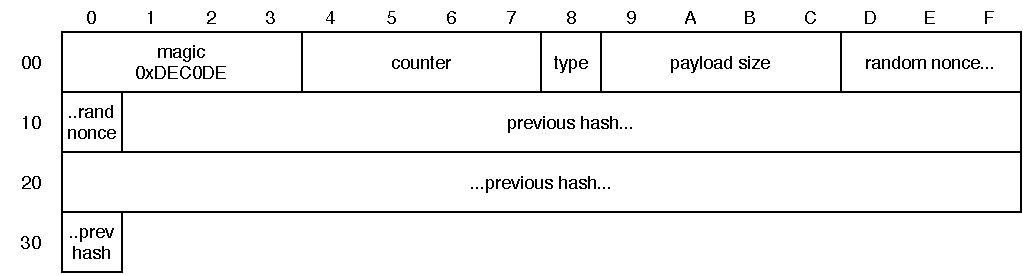
\includegraphics[width=\textwidth]{header}
	\caption{Header format}\label{fig:header}
\end{figure}

\begin{enumerate}
	\item Alice sends to the Server the \code{CLIENT\_HELLO} message shown
		in~\figref{fig:client-hello};
	\item The server sends to Alice its certificate (not shown, just a plain
		message with the certificate);
	\item The server sends to Alice the \code{SERVER\_HELLO} message shown
		in~\figref{fig:server-hello};
	\item Alice and the Server exchange their Diffie-Hellman public keys
		with the messages shown in~\figref{fig:alice-dhkey} and
		\figref{fig:server-dhkey};
	\item Alice sends to the Server the \code{PLAYER\_LIST\_REQ} message
		shown in~\figref{fig:player-list-req};
	\item The server responds to Alice with the \code{PLAYER\_LIST} mssage
		shown in~\figref{fig:player-list};
	\item Alice sends to the Server the \code{CHALLENGE\_REQ} message shown
		in~\figref{fig:challenge-req} saying that she wants to challenge
		Bob;
	\item The Server forwards the request to Bob. The message sent by the
		Server is a \code{CHALLENGE\_REQ} message similar to the one
		shown in~\figref{fig:challenge-req}, the only difference is that
		the \code{username} field contains ``Alice'' instead of ``Bob''
		and all the header's fields are recomputed according to the
		protocol;
	\item Bob (which is already logged-in with the server) responds with the
		\code{CHALLENGE\_RES} message shown
		in~\figref{fig:challenge-res} to accept the challenge;
	\item The Server forwards the \code{CHALLENGE\_RES} message to Alice.
		Then, it sends to Alice a \code{CLIENT\_INFO} message containing
		the necessary informations to allow Alice to connect with Bob
		and sends to Bob another \code{CLIENT\_INFO} message with the
		necessary informations to allow Bob to connect with Alice. The
		format of the \code{CLIENT\_INFO} message is shown
		in~\figref{fig:client-info};
	\item Alice and Bob exchange their Diffie-Hellman public keys with the
		\code{DHKEY} message shown in~\figref{fig:alice-dhkey-p2p}. The
		figure shows only the message sent by Alice to Bob: the message
		sent by Bob to Alice is the same (except that the key is
		different and all the header's fields are recomputed according
		to the protocol);
	\item Alice and Bob can now play their game. They exchange their moves
		using the \code{GAME\_MOVE} message shown
		in~\figref{fig:game-move}.
\end{enumerate}

\begin{figure}[htb]
	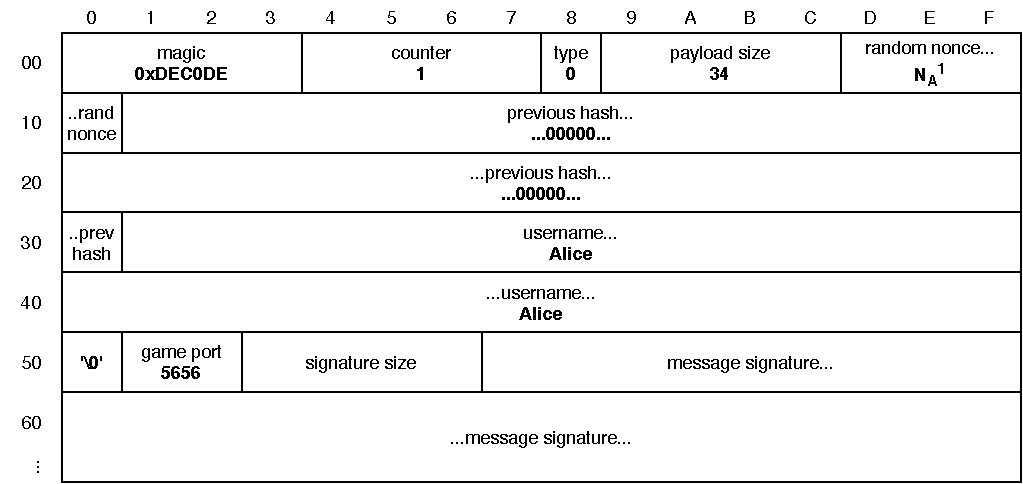
\includegraphics[width=\textwidth]{client-hello}
	\caption{\code{CLIENT\_HELLO} message format}\label{fig:client-hello}
\end{figure}

\begin{figure}[htb]
	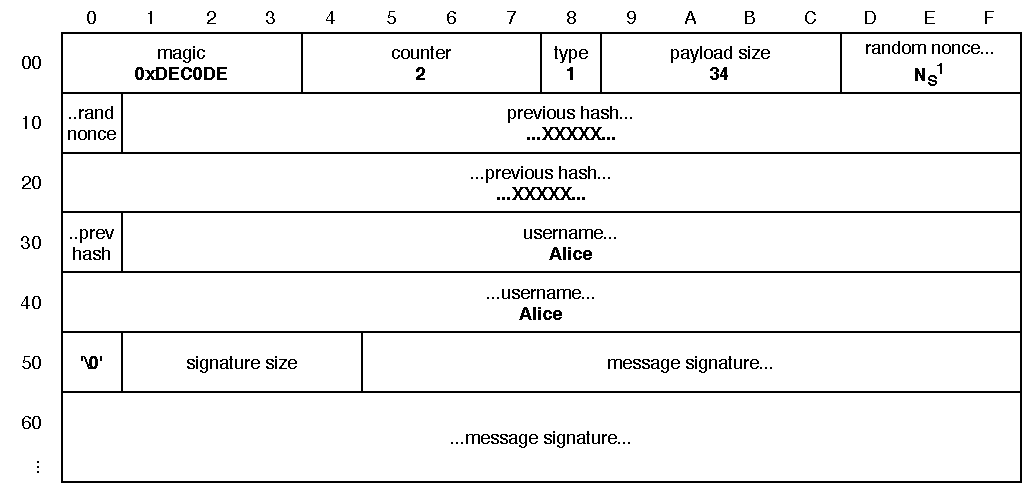
\includegraphics[width=\textwidth]{server-hello}
	\caption{\code{SERVER\_HELLO} message format}\label{fig:server-hello}
\end{figure}

\begin{figure}[htb]
	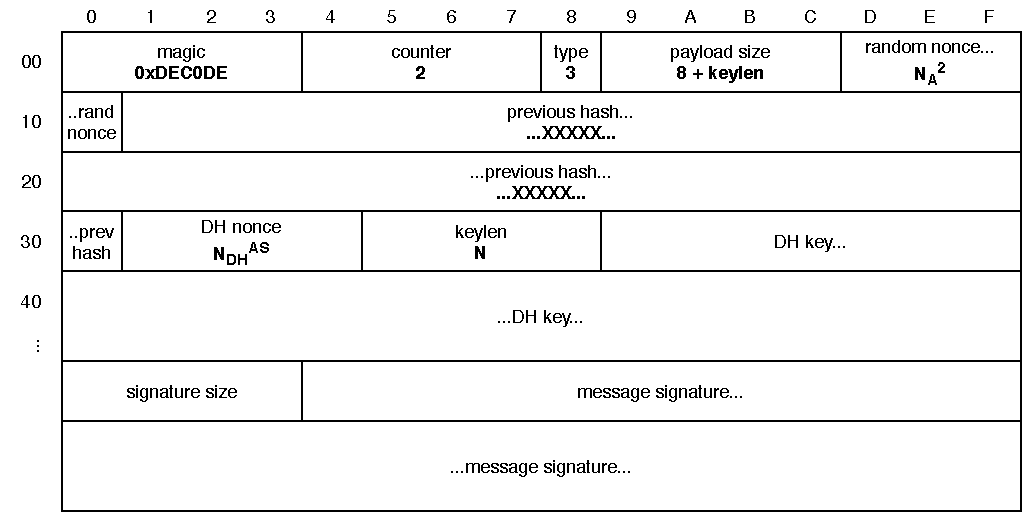
\includegraphics[width=\textwidth]{alice-dhkey}
	\caption{\code{DHKEY} message format sent by Alice}\label{fig:alice-dhkey}
\end{figure}

\begin{figure}[htb]
	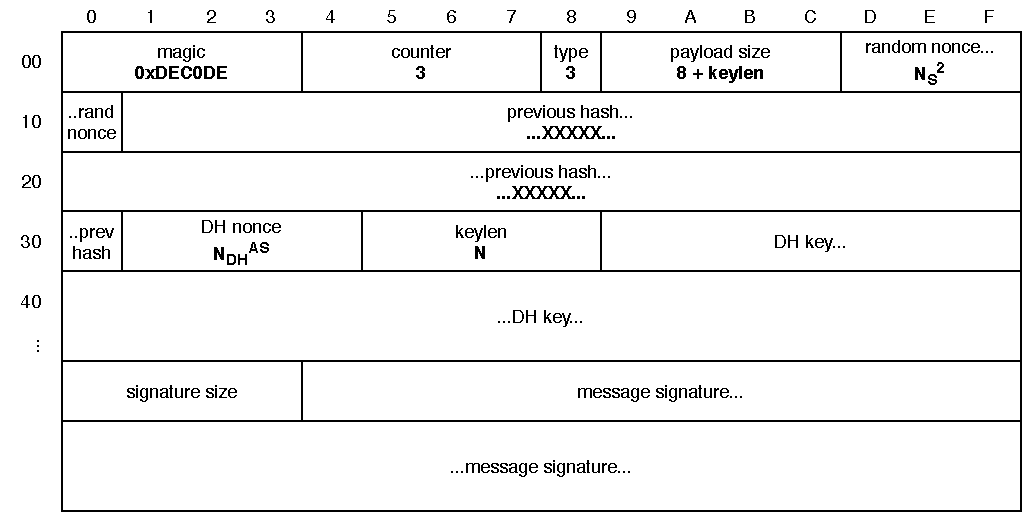
\includegraphics[width=\textwidth]{server-dhkey}
	\caption{\code{DHKEY} message format sent by the Server}\label{fig:server-dhkey}
\end{figure}

\begin{figure}[htb]
	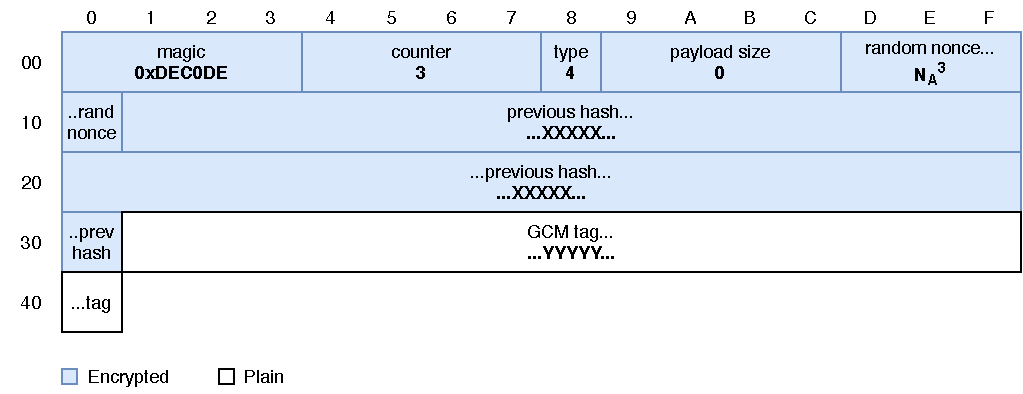
\includegraphics[width=\textwidth]{player-list-req}
	\caption{\code{PLAYER\_LIST\_REQ} message format}\label{fig:player-list-req}
\end{figure}

\begin{figure}[htb]
	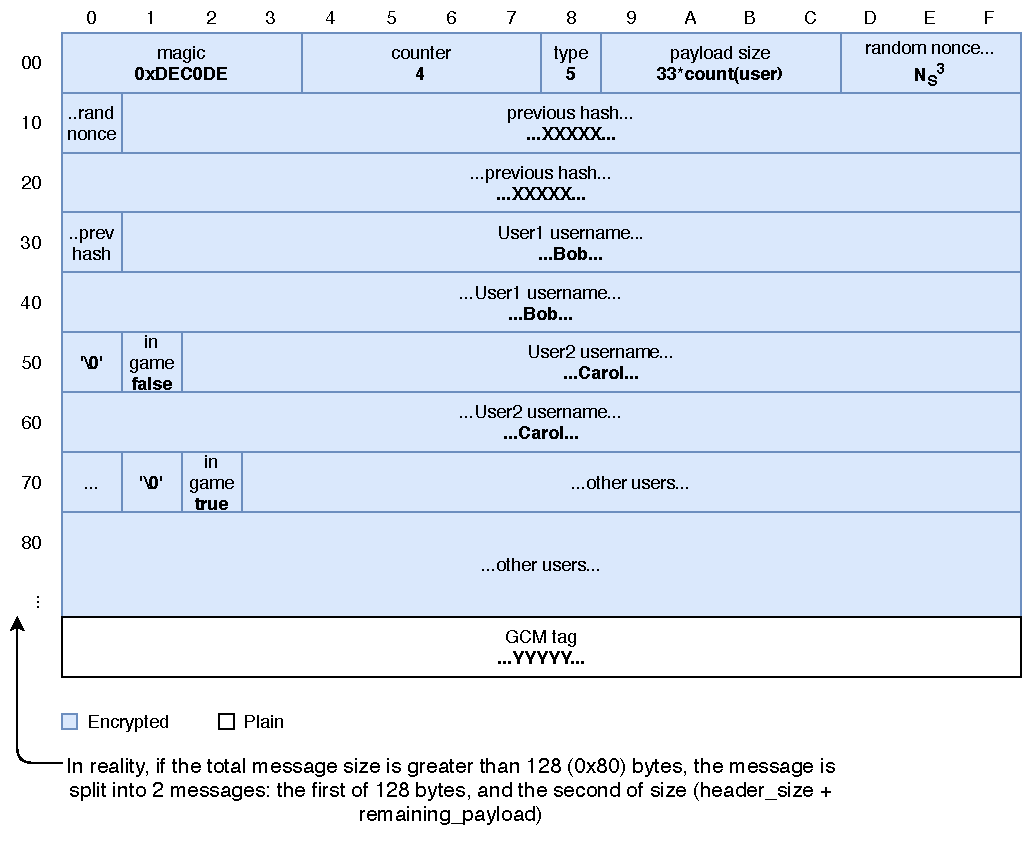
\includegraphics[width=\textwidth]{player-list}
	\caption{\code{PLAYER\_LIST} message format}\label{fig:player-list}
\end{figure}

\begin{figure}[htb]
	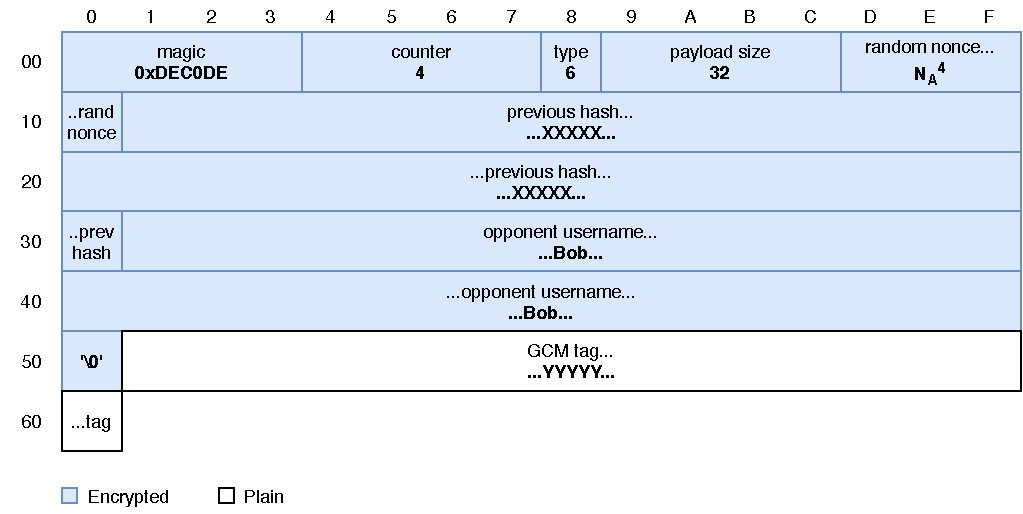
\includegraphics[width=\textwidth]{challenge-req}
	\caption{\code{CHALLENGE\_REQ} message format}\label{fig:challenge-req}
\end{figure}

\begin{figure}[htb]
	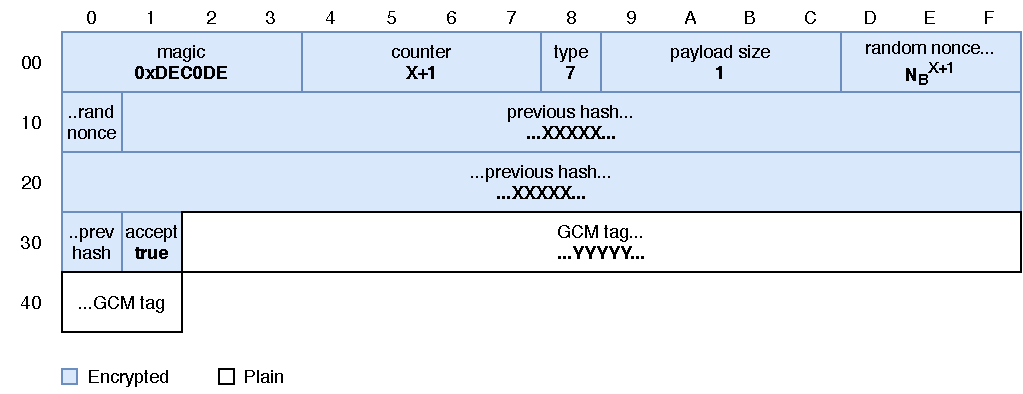
\includegraphics[width=\textwidth]{challenge-res}
	\caption{\code{CHALLENGE\_RES} message format}\label{fig:challenge-res}
\end{figure}

\begin{figure}[htb]
	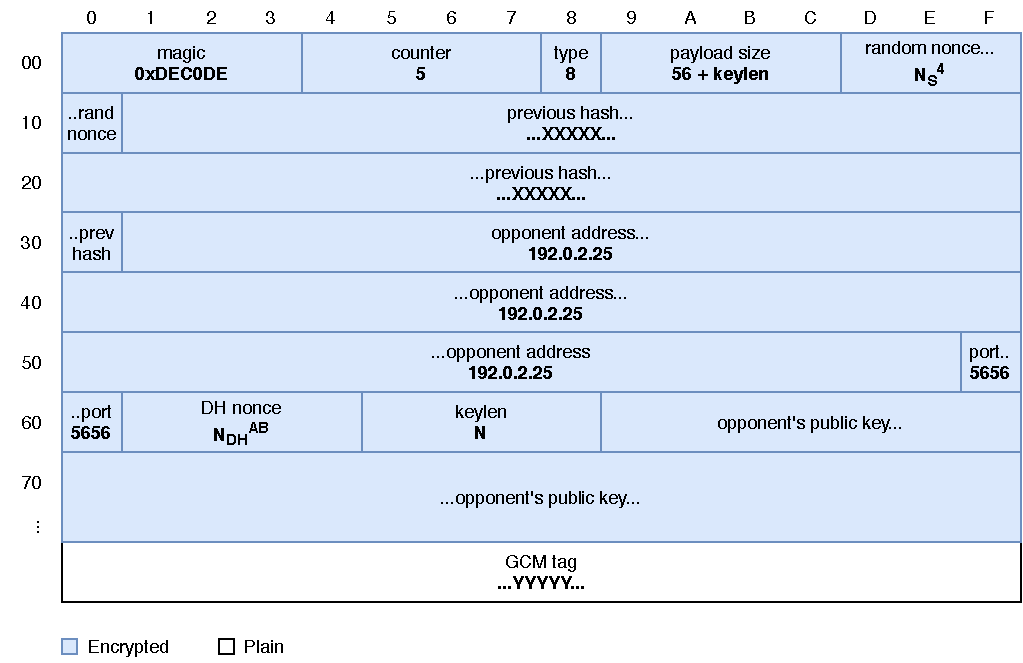
\includegraphics[width=\textwidth]{client-info}
	\caption{\code{CLIENT\_INFO} message format}\label{fig:client-info}
\end{figure}

\begin{figure}[htb]
	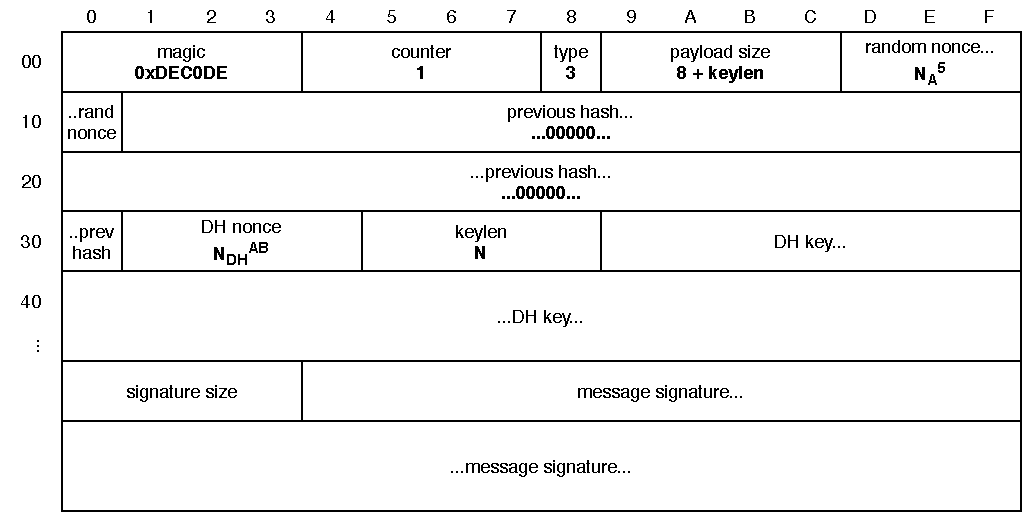
\includegraphics[width=\textwidth]{alice-dhkey-p2p}
	\caption{\code{DHKEY} message format sent by Alice to Bob}\label{fig:alice-dhkey-p2p}
\end{figure}

\begin{figure}[htb]
	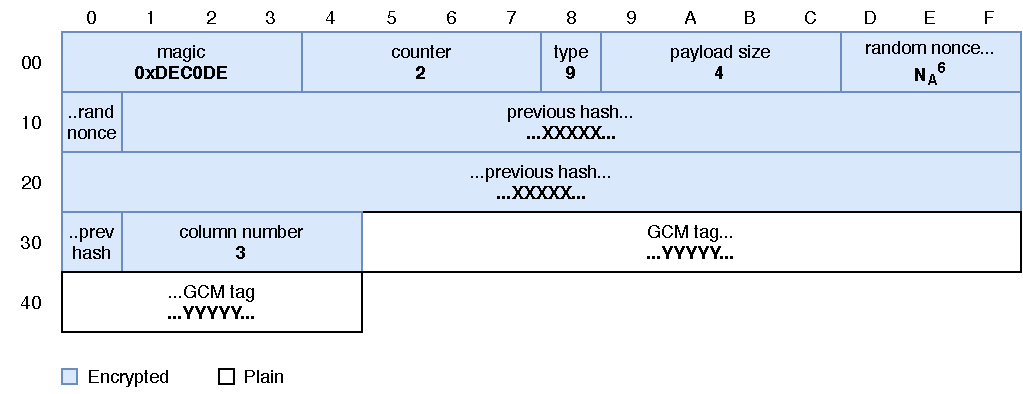
\includegraphics[width=\textwidth]{game-move}
	\caption{\code{GAME\_MOVE} message format}\label{fig:game-move}
\end{figure}
